\documentclass[14pt,a4paper,oneside]{extbook}
\usepackage[utf8]{inputenc}
\usepackage[russian]{babel}
\usepackage{fancyhdr}
\usepackage{amsmath}
\usepackage{amsfonts}
\usepackage{amssymb}
\usepackage{dsfont}
\usepackage{mathrsfs}
\usepackage{comment}
\usepackage{graphicx}
\usepackage{pgfplots}
\usepackage{xparse}
\usepackage{listings}
\usepackage{longtable}
\usepackage{tabto}
\usepackage[left=2cm,right=2cm,top=2cm,bottom=2cm]{geometry}
\usepackage{alltt}
\usepackage[numbers,sort&compress]{natbib}
\usepackage{hyperref}
\usepackage{datetime}
\usepackage{tcolorbox}

\usepackage{tabularx}
\usepackage{graphicx}
\newcolumntype{L}[1]{>{\hsize=#1\hsize\raggedright\arraybackslash}X}%
\newcolumntype{R}[1]{>{\hsize=#1\hsize\raggedleft\arraybackslash}X}%
\newcolumntype{C}[1]{>{\hsize=#1\hsize\centering\arraybackslash}X}%

\newcommand{\T}{\rule{0pt}{2.3ex}} %top strut
\newcommand{\B}{\rule[-1.2ex]{0pt}{0ex}} %bottom strut

\newcommand{\sexstar}{{\fontfamily{lmr}\selectfont$\star$}}
\newcommand*{\expect}{\mathsf{M}}
\newcommand*{\prob}{\mathsf{P}}

\usepackage[section, above, below]{placeins}

\usepackage{titlesec}
\setcounter{tocdepth}{2}
\newcommand{\chn}{{{}{\arabic{chapter}.}}}
\titleformat{\chapter}[block]{\bfseries\raggedright\hyphenpenalty=2000}
{\LARGEДомашнее задание \arabic{chapter}.}{1ex}{\rule{\linewidth}{1pt}\newline\Large}

\titleformat{\section}[block]{\bfseries\raggedright\hyphenpenalty=10000}
{\arabic{section}.}{1ex}{}
\titleformat{\subsection}[block]{\bfseries\normalsize\raggedright\hyphenpenalty=10000}
{\chn\arabic{section}.\arabic{subsection}.}{1ex}{}
\titleformat{\subsubsection}[block]{\bfseries\normalsize\raggedright\hyphenpenalty=10000}
{\chn\arabic{section}.\arabic{subsection}.\arabic{subsubsection}.}{1ex}{}
\addto\captionsrussian{\renewcommand{\chaptername}{Задание}}
\titlespacing*{\chapter}      {0pt}{3.50ex plus 1ex minus .2ex}{2.3ex plus .2ex}
\titlespacing*{\section}      {0pt}{3.50ex plus 1ex minus .2ex}{2.3ex plus .2ex}
\titlespacing*{\subsection}   {0pt}{3.25ex plus 1ex minus .2ex}{1.5ex plus .2ex}
\titlespacing*{\subsubsection}{0pt}{3.25ex plus 1ex minus .2ex}{1.5ex plus .2ex}

%\sloppy

\renewcommand{\labelitemi}{$\triangleright$}



\newcounter{rownum}
\setcounter{rownum}{0}
\newcommand{\Rownum}{\stepcounter{rownum}%
	\arabic{rownum}}


\usepackage{catchfile,environ,tikz}

\newcounter{tablinegen}
\newcounter{tabrow}
\newcommand{\nl}{\stepcounter{tabrow}\\ \hline}
\newcommand{\blankline}{\thetabrow & \nl}
\newcommand{\blanklist}[3][.8\textwidth]{% #1 - names
	\begingroup
	\setcounter{tablinegen}{0}
	\let\tablines\empty%
	\loop\ifnum\thetablinegen<#2
	\stepcounter{tablinegen}
	\expandafter\def\expandafter\tablines\expandafter{%
		\tablines
		\blankline
	}%
	\repeat
	\blanklistformat{#1}}
\newcommand{\blanklistformat}[1]{
	\renewcommand{\arraystretch}{1.5}
	\begin{tabular}{|>{\raggedright\arraybackslash}X|>{\raggedright\arraybackslash}X|>{\raggedright\arraybackslash}X|}
		\hline
		ФИО & Дискретное распределение & Непрерывное распределение  \nl
		\tablines
	\end{tabular}
	\endgroup
	\setcounter{tabrow}{0}}


\usepackage{catchfile,environ,tikz}


\begin{document}
	
	
	\begin{titlepage}                                                         
		\newpage                                                                        
		\begin{center}                                                        
			{\bfseries Национальный Исследовательский Университет \\
				Высшая Школа Экономики \\
				Московский Институт Электроники и Математики}                               
			\vspace{1cm}                                                          
			%САНКТ-ПЕТЕРБУРГСКИЙ \\*                                                
			%ГОСУДАРСТВЕННЫЙ УНИВЕРСИТЕТ \\*                                        
			%\hrulefill                                                                     
			%\end{center}                                                         
			
			%{КАФЕДРА ЯДЕРНОЙ ФИЗИКИ }                                 
			Департамент Прикладной Математики
			
			Кафедра Компьютерной Безопасности                                                              
			\vspace{6em}                                                          
			
			
			
			
			
			
			
		\end{center}                                                          
		
		\vspace{1.2em}                                                        
		
		\begin{center}                                                        
			%\textsc{\textbf{}}                                     
			\Large Долгосрочное домашнее задание по математической
			статистике\linebreak                                  
			
			
		\end{center}                                            
		\begin{center}
			\textbf{Дискретное распределение:}\textit{ Биномиальное распределение $n = 87, \theta = 0.6$}\\
			\textbf{Равномерное распределение:} \textit{ Распределение Максвелла $\theta = 3$}
		\end{center}
		
		\vspace{5em}                                                          
		
		\begin{center}                                                        
			%\Large                                                                         
			
		\end{center}                                                         
		\vspace{6em}                                                          
		
		%\begin{center}                                                   
		%\begin{tabbing}                                                      
		
		\quad\tabto{320pt}Выполнил \\                                     
		\tabto{320pt}Смирнов Д. А.\\                                           
		\vspace{1.2em}                                                       
		\tabto{320pt}Проверил \\                                                      
		\tabto{320pt}Чухно А. Б.\\                                        
		%\end{tabbing}                                                        
		%\end{center}                                                         
		\begin{comment}                          
		\begin{alltt}                                                         
		Научный руководитель                                             
		Рґ.С„.Рј.РЅ., Andrey Р’.Рђ.                                            
		Рецензент                                                        
		к.ф.-м.н. Olegovich В.И.                                         
		\end{alltt}                                             
		\end{comment}                                                                                        
		
		\vspace{\fill}                                                    
		
		\begin{center}                                                        
			Москва \the\year{}                                                                
		\end{center}                                                          
	\end{titlepage}
	\setcounter{page}{2}
	\tableofcontents
	
	\chapter{Характеристики вероятностных распределений}
	
	\underline{\textbf{Описание основных характеристик распределений}}
	\section{Биномиальное распределение}
	$\displaystyle P(x) = \binom{n}{x}\theta^{x}(1-\theta)^{n-x}, x \in \{0, 1, ..., n\}, n \in \mathbb {N}, 0 < \theta < 1$ 
	
	\subsection{Функция Распределения}
	В общем виде функция распределения Биномиального распределения выглядит следующим образом [\textit{\textbf{1} - Фомин Д. Б, Чухно А. Б., "Теория вероятности. Курс лекций для студентов кафедры компьютерной безопасности", МИЭМ НИУ ВШЭ, Москва 2022: \textbf{стр. 90}}]: \\
	$F(x) = P(\xi < x) = \displaystyle\sum_{k=0}^{x} \binom{n}{x}\theta^{k}(1-\theta)^{n-k}, x \in \{0,1,...,n\}, n \geq 1, 0 < \theta < 1$
	
	\subsection{Математическое ожидание}
	По определению, математическое ожидание дискретной случайной величины вычисляется по формуле [\textit{\textbf{2} - Фомин Д. Б, Чухно А. Б., "Теория вероятности. Курс лекций для студентов кафедры компьютерной безопасности": \textbf{стр. 63}}]: \\
	$\displaystyle M\xi = \displaystyle\sum_{i\geq1}x_i \cdot p_i$, где $p_i = P(\xi = x_i)$ \\
	Пусть случайная величина $\xi$ имеет биномиальное распределение с параметрами $(n, \theta)$, что соответствует числу успехов в $n$ независимых испытаниях Бернулли с вероятностю успеха $\theta$ в каждом испытании [\textit{\textbf{3} - Фомин Д. Б, Чухно А. Б., "Теория вероятности. Курс лекций для студентов кафедры компьютерной безопасности": \textbf{стр. 67}}]. \\
	Представим $\xi$ в виде суммы $n$ независимых индикаторов $\chi_1,...,\chi_n$, где $\chi_i = 1$, если в $i$-ом испытании Бернулли произошел успех. \\
	Имеем: $\displaystyle P(\chi_i = 1) = \theta, P(\chi_i = 0) = 1 - \theta, i \in \overline{1,n}$ \\
	Тогда: $\displaystyl M\xi = M(\displaystyle\sum_{i = 1}^{n}\chi_i) = \displaystyle\sum_{i=1}^{n}M\chi_i = n\theta$
	
	\subsection{Дисперсия}
	По определению, Дисперсия $D\xi = M(\xi - M\xi)^2 = M\xi^2 - (M\xi)^2$ [\textit{\textbf{4} - Фомин Д. Б, Чухно А. Б., "Теория вероятности. Курс лекций для студентов кафедры компьютерной безопасности": \textbf{стр. 71}}] \\
	Также по \textit{\textbf{Определению 7.5}} [\textit{\textbf{5} - Фомин Д. Б, Чухно А. Б., "Теория вероятности. Курс лекций для студентов кафедры компьютерной безопасности": \textbf{стр. 71}}] знаем, что для дискретной случайной величины \\
	$\displaystyle M(\xi - M\xi)^{n} = \displaystyle\sum_{k=1}^{n}(x_k - M\xi)^{n} \cdot P(\xi = x_k)$ \\
	Тогда: $D\xi = \displaystyle\sum_{k = 1}^{n=2}(\chi_k - M\xi)^2 \cdot p_k$. С учетом функции распределения из пункта \textbf{1.1.1}, получаем, что \\
	$D\xi = \displaystyle\sum_{k = 1}^{n=2}(\chi_k - M\xi)^2 \cdot p_k = \displaystyle\sum_{x=0}^{n=2}(x - n \cdot \theta)^{2} \cdot \binom{n}{x} \cdot \theta^{x} \cdot (1 - \theta)^{n - x} = n \cdot \theta \cdot (1 - \theta)$
	
	\subsection{Квантиль уровня $\gamma$}
	$\gamma$-квантиль - это такое значение $\chi$ случайной величины $\Chi$, для которого $P(\Chi \leq \chi \cdot \gamma) = \gamma$. То есть, вероятность того, что случайная величина $\Chi$ примет значение меньше или равное $x$ [\textit{\textbf{6} - \href{https://allatambov.github.io/psms/pdf/quantiles.pdf}{Источник}}]\\
	$\displaystyle\sum_{k=1}^{x} \binom{n}{x} \theta^{k} \cdot (1 - \theta)^{n - k} = \gamma$
	
	\subsection{Пример интерпритации распределения}
    Биномиальное распределение - распределение количества «успехов» в последовательности из $n$ независимых случайных экспериментов, таких что вероятность «успеха» в каждом из них равна $\theta$. [\textit{\textbf{7} - \href{https://ru.wikipedia.org/wiki/Биномиальное_распределение}{Источник}}] Такая схема испытаний (экспериментов) называется схемой испытаний Бернулли. [\textit{\textbf{8} - \href{https://ru.wikipedia.org/wiki/Схема_Бернулли}{Источник}}]\\ 
    Примеры:
    \begin{enumerate}
        \item \textbf{Контроль качества изделий} [\textit{\textbf{9} - \href{https://studopedia.ru/5_19612_primenenie-binomialnogo-raspredeleniya.html}{Источник}}] \\
        Каждое изделие с вероятностью $\theta$ может быть дефектным. Появление как дефектных, так и стандартных изделий происходит независимо друг от друга. \\
        \textit{Пример:} \\
        Дано: $n = 87 изделий, \theta = 0.6 - $ вероятность того, что изделие "стандартно" \\
        Решение: Случайная величина $\xi$ распределена по Биномиальному закону с вышеописанными параметрами. Воспользуемся формулой Бернулли: \\
        $\displaystyle P(\xi = x) = P_{n}(x) = \binom{n}{x}\theta^{x}(1-\theta)^{n - x} = \binom{87}{x}0.6^{x}(1-0.6)^{87 - x} = \frac{87!}{x!(87 - x)!} \cdot 0.6^{x} \cdot 0.4^{87 - x}, x = 0, 1, 2, \cdots, 87$ \\
        С помощью скрипта на языке Python составим таблицу, описывающую ряд распределения: \\
        \begin{figure}[h]
        \centering
        \fbox{\includegraphics[scale=1]{HW1/Binomial/Examples/Details/1.png}
        \includegraphics[scale=1]{HW1/Binomial/Examples/Details/2.png}}
        \caption{}
        \label{fig:my_label}
    \end{figure}
        \newpage
        \item \textbf{Телекоммуникации} [\textit{\textbf{10} - \href{http://statistica.ru/theory/binomialnoe-raspredelenie/}{Источник}}] \\
        Здесь $(1 - \theta)$ - доля необслуженных вызовов. \\
        Пример для данной интерпритации анологичен примеру, описанному выше.
    \end{enumerate}
    \subsection{Соотношения между распределениями} [\textit{\textbf{11} - \href{https://ru.wikipedia.org/wiki/Биномиальное_распределение#Связь_с_другими_распределениями}{Источник}}]
    \begin{enumerate}
        \item Если $n = 1$, то получаем распределение Бернулли.
        \item Если $n$ большое, то в силу центральной предельной теоремы [\textit{\textbf{12} - Фомин Д. Б, Чухно А. Б., "Теория вероятности. Курс лекций для студентов кафедры компьютерной безопасности": \textbf{стр. 124}}] \\ $Bin(n, \theta) \approx N(n\theta, n\theta(1-\theta))$, где $N(n\theta, n\theta(1-\theta))$ - нормальное распределение с $M\xi = n\theta$ и $D\xi = n\theta(1-\theta)$.
        \item Если $n$ - большое, а $\lambda$ - фиксированное число, то $Bin(n, \frac{\lambda}{n}) \approx P(\lambda)$, где $P(\lambda)$ - распределение Пуассона с параметром $\lambda$. 
    \end{enumerate}
    
    \subsection{Описание способа моделирования выбранных случайных величин}
    [\textit{\textbf{13} - \href{http://statmod.ru/wiki/_media/books:vv:simulation_v4.pdf}{Источник, \textbf{стр. 26}}}] Биномиальное распределение $Bin(n, \theta)$ с параметрами $n \in \mathbb{N} \textrm{и} \theta \in (0,1)$ можно задать с помощью \textbf{таблицы распределения:} \\
    $
        P:
        \begin{pmatrix}
            0 & 1 & \cdots & k & \cdots & n \\
            \theta_{0} & \theta_{1} & \cdots & \theta_{k} & \cdots & \theta_{n}
        \end{pmatrix}
    $
	, где $\theta_{k} = \binom{n}{k} \theta^{k} (1 - \theta)^{n - k}.$ \\
	Воспользуемся последовательным методом набором обратных функций в нетабличном варианте. Накопленные вероятности $s_{k}$ здесь вычисляются в том же цикле, где проверяются неравенства $\alpha \leq s_{k}$. То есть вероятности $\theta_{k}$ рекуррентно пересчитываются одна через другую, а накопленные вероятности $s_{k}$ последовательно вычисляются через $s_{k-1} \textrm{и} \theta_{k}$ \\
	Для биномиального распределения $\theta_{0} = (1 - \theta)^{n} \textrm{ и }$ \\
	\begin{center}
	$\displaystyle\frac{\theta_{k}}{\theta_{k-1}} = \frac{n - k + 1}{k} \frac{\theta}{1 - \theta}$
	\end{center}
	\\
	при $k = 1, 2, \cdots, n, \textrm{то мы приходим к алгоритму BIS (Binomial Inverse Sequential).}$ Однако, воспользуемся мы алгоритмом BISM: заметим, что если $\xi \in Bin(n, \theta), \\ \textrm{ то } \eta = n - \xi \in Bin(n, 1 - \theta).$ Поэтому, если $\theta > 0.5$, то можно применить алгоритм BIS к моделированию числа неудач в $n$ испытаниях Бернулли с вероятностью
    успеха $\theta$, а потом перейти к числу успехов, что равносильно применению последовательного метода обратных функций «справа налево», а не «слева направо». \\
    Далее описан \textbf{Алгоритм BISM (Binomial Inverse Sequential Modified)}: \\
    \begin{center}
	Моделирование $Bin(n, \theta)$ модифицированным последовательным методом обратных функций.
	\end{center} \\
	Входные данные: $n, \theta$ \\
	Результат: $\xi$. \\
	\textbf{1. Инициализация}
	\begin{itemize}
	    \item $\textrm{If } \theta \leq 0.5 \textrm{ then } t \longleftarrow \theta \textrm{ else } t \longleftarrow 1 - \theta;$
	    \item $c \longleftarrow t/(1 - t); s \longleftarrow r \longleftarrow (1 - t)^{n}; k \longleftarrow 0; Get(\alpha);$
	\end{itemize}
	\\
	\textbf{2. Пересчет вероятностей и поиск окна}
	\begin{itemize}
	    \item $k \longleftarrow k + 1; r \longleftarrow r \cdot c \cdot (n - k + 1)/k; s \longleftarrow s + r;$
	\end{itemize}
	\\
	\textbf{2. Завершение: } $\textrm{If } p \leq 0.5 \textrm{ then } \xi \longleftarrow k \textrm{ else } \xi \longleftarrow n - k; \textrm{ STOP. }$
	\\
	Комментария требует лишь введение переменной $t$, которая необходима при завершении алгоритма, чтобы (если нужно) перейти от моделирования числа неудач в испытаниях Бернулли к
    моделированию числа успехов. \\
    В процессе выполнения Домашнего Задания мною была разработана программа на языке Python, моделирующая 10000 случайных величин с Биномиальным распределением и строющая график плотности вероятности. Параметры: $n = 87, \theta = 0.6$ \\
    \textbf{\textit{График:}}
    \begin{center}
         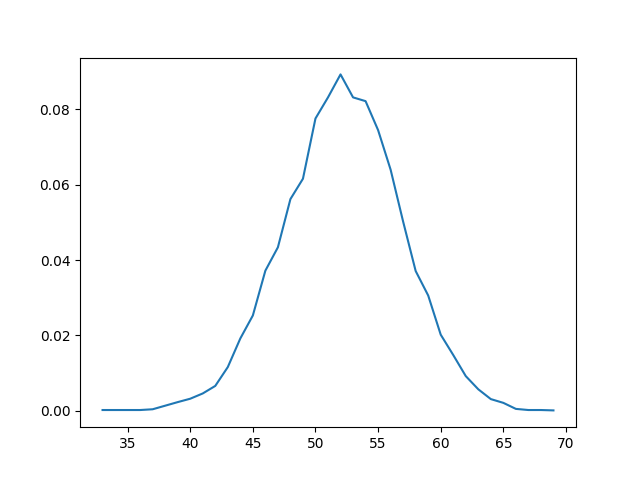
\includegraphics[scale=1.2]{HW1/Binomial/3_Model/Binomial.png}
    \end{center}

    \\
    \textbf{\textit{Листинг кода:}}
    \lstinputlisting[language=Python]{HW1/Binomial/3_Model/binomial.py}
	\newpage
	\section{Распределение Максвелла}
	$\displaystyle f(x) = \sqrt{\frac{2}{\pi}} \frac{x^{2}}{\theta^{3}} e^{-\frac{x^{2}}{2\theta^{2}}}, x, \theta \in \mathbb{R^{+}}$
	\subsection{Функция Распределения}
	По определению [\textit{\textbf{14} - Фомин Д. Б, Чухно А. Б., "Теория вероятности. Курс лекций для студентов кафедры компьютерной безопасности": \textbf{стр. 52}}], функция распределения непрывного распределения вычисляется по формуле: \\
	$\displaystyle F(x) = \int\limits_{-\infty}^{x}f(t)\mathrm{d}t$. Тогда:

    $F_{\xi}(x) = \int\limits_{-\infty}^{x} f(t) \,\mathrm{d}t = \int\limits_{-\infty}^{x} \displaystyle \sqrt{\frac{2}{\pi}}\frac{t^2}{\theta^3} e^{-\frac{t^2}{2\theta^2}}\,\mathrm{d}t = \displaystyle \sqrt{\frac{2}{\pi}}\frac{1}{\theta^3} \int\limits_{-\infty}^{x} t^2 e^{-\frac{t^2}{2\theta^2}}\,\mathrm{d}t  =$ \\ опираясь на то, что $d(e^{-\frac{t^2}{2\theta^2}})= -\frac{t e^{-\frac{t^2}{2\theta^2}}}{\theta^2}\,\mathrm{d}t,$ получим $= 
    \displaystyle -\sqrt{\frac{2}{\pi}}\frac{1}{\theta^3}\theta^2 \int\limits_{-\infty}^{x} \frac{t^2}{t}\,d(e^{-\frac{t^2}{2\theta^2}}) = \displaystyle -\sqrt{\frac{2}{\pi}}\frac{1}{\theta} \int\limits_{-\infty}^{x}t\,d(e^{-\frac{t^2}{2\theta^2}}) =$ возьмем интеграл по частям $= \displaystyle -\sqrt{\frac{2}{\pi}}\frac{1}{\theta}(t e^{-\frac{t^2}{2\theta^2}}\bigg|_{-\infty}^{x} -- \int\limits_{-\infty}^{x} e^{-\frac{t^2}{2\theta^2}}\,\mathrm{d}t) = \displaystyle -\sqrt{\frac{2}{\pi}}\frac{1}{\theta}x e^{-\frac{x^2}{2\theta^2}} + \sqrt{\frac{2}{\pi}}\frac{1}{\theta}\theta\sqrt{2\pi}\int\limits_{-\infty}^{x} \frac{1}{\theta\sqrt{2\pi}}^{-\frac{t^2}{2\theta^2}}\,\mathrm{d}t) =$\\так как $x,\theta \in \mathbb{R^{+}} =\displaystyle -\sqrt{\frac{2}{\pi}}\frac{1}{\theta}x e^{-\frac{x^2}{2\theta^2}} + \sqrt{\frac{2}{\pi}}\frac{1}{\theta}\theta\sqrt{2\pi}\int\limits_{0}^{x} \frac{1}{\theta\sqrt{2\pi}}^{-\frac{t^2}{2\theta^2}}\,\mathrm{d}t) =$\\ видно, что правое слагаемое есть функция плотности стандартного нормального распределения $= \displaystyle -\sqrt{\frac{2}{\pi}}\frac{1}{\theta}x e^{-\frac{x^2}{2\theta^2}} + 2\int\limits_{0}^{x} f_N(t)\,\mathrm{d}t  =\displaystyle -\sqrt{\frac{2}{\pi}}\frac{1}{\theta}x e^{-\frac{x^2}{2\theta^2}} + 2 F_N(x)$
    
    Здесь $F_N(x)$ - функция распределения N(0,1).\vspace{0.7in}
    
	\subsection{Математическое ожидание}
	По определению [\textit{\textbf{15} - Фомин Д. Б, Чухно А. Б., "Теория вероятности. Курс лекций для студентов кафедры компьютерной безопасности": \textbf{стр. 68}}], Математическое ожидание непрерывной случайной величины $\xi$ вычисляется по формуле: \\
	$M\xi = \int_{-\infty}^{+\infty}x\mathrm{d}F_{\xi}(x)$. Тогда: \\
	\begin{multline*}
    M\xi = \int\limits_\mathbb{R} x f\xi(x)\mathrm{d}x= \int\limits_{-\infty}^{+\infty}x \sqrt{\frac{2}{\pi}} \frac{x^2}{\theta^3}\exp(-\frac{x^2}{2\theta^2})\mathrm{d}x = \sqrt{\frac{2}{\pi}} \frac{1}{\theta^3} \int\limits_{-\infty}^{+\infty} x^3\exp(-\frac{x^2}{2\theta^2})\mathrm{d}x =\\=\textrm{так как }x,\theta \in \mathbb{R}^+, \textrm{ то} = \sqrt{\frac{2}{\pi}} \frac{1}{\theta^3} \int\limits_{0}^{+\infty} x^3\exp(-\frac{x^2}{2\theta^2})\mathrm{d}x \end{multline*}
    Для упрощения работы, сначала вычислим неопределённый интеграл:
    \begin{multline*}
    \int x^3\exp(-\frac{x^2}{2\theta^2})\mathrm{d}x = \textrm{Произведём замену вида } u = x^{2}x^2, \textrm{ тогда } \mathrm{d}x = \frac{1}{2x}\mathrm{d}u = \\ = \frac{1}{2} \int u\exp(-\frac{u}{2\theta^2})\mathrm{d}u = \textrm{Произведём замену вида } v = -\frac{u}{2\theta^2}, \textrm{ тогда } \mathrm{d}u = -2\theta^2 d v =\\= 2\theta^4 \int v e^v \mathrm{d}v = \textrm{Возьмём интеграл по частям} =2\theta^4 (v e^v - \int e^v \mathrm{d}v) = 2\theta^4 (v e^v -  e^v) = \\ = \textrm{Выполним обратную замену} = -(\theta^2x^2 + 2\theta^4)\exp(-\frac{x^2}{2\theta^2}) + \mathbb{C}
    \end{multline*}
    Таким образом:
    $$-(\theta^2x^2 + 2\theta^4)\exp(-\frac{x^2}{2\theta^2}) \bigg|_{0}^{+\infty}  = 2\theta^4$$
    Следовательно, математическое ожидание равно: $\displaystyle \sqrt{\frac{2}{\pi}} \frac{1}{\theta^3}  2\theta^4 = \displaystyle\sqrt{\frac{2}{\pi}} 2\theta $\\
    
	\subsection{Дисперсия}
	По определению, Дисперсия $D\xi = M(\xi - M\xi)^2 = M\xi^2 - (M\xi)^2$ [\textit{\textbf{16} - Фомин Д. Б, Чухно А. Б., "Теория вероятности. Курс лекций для студентов кафедры компьютерной безопасности": \textbf{стр. 71}}] \\
	В пункте \textbf{1.2.2} было выведено $M\xi = \displaystyle\sqrt{\frac{2}{\pi}} 2\theta$, тогда $(M\xi)^2 = \displaystyle \frac{8}{\pi} \theta^2$.\\
    Выведем $M\xi^2$:
    \begin{multline*}
    M\xi^2 = \int\limits_\mathbb{R} x^2 f\xi(x)\mathrm{d}x = \int\limits_{-\infty}^{+\infty}x^2 \sqrt{\frac{2}{\pi}} \frac{x^2}{\theta^3}\exp(-\frac{x^2}{2\theta^2})\mathrm{d}x = \sqrt{\frac{2}{\pi}} \frac{1}{\theta^3} \int\limits_{-\infty}^{+\infty} x^4\exp(-\frac{x^2}{2\theta^2})\mathrm{d}x =\\=\textrm{так как }x,\theta \in \mathbb{R}^+, \textrm{ то} = \sqrt{\frac{2}{\pi}} \frac{1}{\theta^3} \int\limits_{0}^{+\infty} x^4\exp(-\frac{x^2}{2\theta^2})\mathrm{d}x =\end{multline*}
    = это следующий интеграл
    \begin{multline*}
     \int\limits_{0}^{+\infty} x^n\exp(-\alpha x^2)\mathrm{d}x = 
    \begin{cases}
    \displaystyle\frac{(2k-1)!!}{2^{k+1}\alpha^k}\sqrt{\frac{\pi}{\alpha}} & \textrm{если } n = 2k, k \in \mathbb{N} , \alpha > 0\\
    \displaystyle\frac{k!}{2\alpha^{k+1}}  & \textrm{если } n = 2k+1, k \in \mathbb{N} , \alpha > 0 
    \end{cases}
      =\\=  \sqrt{\frac{2}{\pi}} \frac{1}{\theta^3} \frac{3}{8} \sqrt{\pi} (2\theta^2)^{2.5}  = 3\theta^2
    \end{multline*}
    Таким образом, получаем дисперсию:
    $$D\xi = M(\xi-M\xi)^2 = M\xi^2 - (M\xi)^2 = 3\theta^2 - \displaystyle \frac{8}{\pi} \theta^2 = \theta^2 (3 - \displaystyle\frac{8}{\pi})$$\\
    
	\subsection{Квантиль уровня $\gamma$}
	По определению: $F\xi(x_\gamma) = \gamma$, значит квантиль распределения - решение уравнения 
    $$\displaystyle -\sqrt{\frac{2}{\pi}}\frac{1}{\theta}x_\gamma \exp(-\frac{x_\gamma^2}{2\theta^2}) + 2 F_N(x_\gamma) = \gamma$$
    Здесь $F_N(x)$ - функция распределения N(0,1)\\
    
    \subsection{Пример интерпритации распределения}
    [\textit{\textbf{17} - \href{https://studopedia.ru/15_37150_raspredelenie-maksvella.html}{Источник}}] Распределение Максвелла (Максвелла-Больцмана) лежит в основе кинетической теории газов, объясняющей многие фундаментальные свойства газов, включая давление и диффузию. Распределение Максвелла применимо к множеству свойств индивидуальных молекул в газе. О нём обычно думают как о распределении энергий молекул в газе, но оно может также применяться к распределению скоростей, импульсов, и модуля импульсов молекул. \\
    \textit{Ниже приведены некоторые примеры интепритации распределения Максвелла в виде функций плотности распределения:}
    \\
    \textbf{Распределение по вектору скорости:}
    [\textit{\textbf{18} - \href{https://ru.wikipedia.org/wiki/Распределение_Максвелла}{Источник}}]
    \begin{center}
        $\displaystyle p = mV \\
        \displaystyle f_{V}(v_{x}, v_{y}, v_{z}) = \sqrt{\Big(\frac{m}{2\pi kT}\Big)^{3}}\cdot exp\Big[\frac{-m(v_{x}^{2}, v_{y}^{2}, v_{z}^{2})}{2kT}\Big]$
    \end{center}
    \newpage
    \textbf{Распределение по проекции скорости:}
    \begin{center}
        $\displaystyle f_{м}(v_{i}) = \sqrt{\frac{m}{2\pi kT}}\cdot exp\Big[\frac{-m v_{i}^{2}}{2kT}\Big]$
    \end{center}
    \textbf{Распределение по модулю импульса:}
    \begin{center}
        $\displaystyle f_{p} = \int\limits_{\theta=0}^{\pi} \int\limits_{\phi=0}^{2\pi}f_{P}p^{2}sin(\theta)d\theta d\phi = 4\pi\sqrt{\Big(\frac{1}{2\pi mkT}\Big)^{3}}\cdot p^{2} \cdot exp\Big[\frac{-p^2}{2mkT}\Big]$
    \end{center}
    \textbf{Распределение по энергии:}
    \begin{center}
        $\displaystyle p^{2} = 2mE \textrm{ и } f_{E}dE = f_{p}dp \\
        \displaystyle f_{E} = f_{p}\frac{dp}{dE} = \frac{2\pi}{\sqrt{(\pi kT)^{3}}}\cdot\sqrt{E}\cdot exp\Big[\frac{-E}{kT}\Big]$
    \end{center}
    [\textit{\textbf{19} - \href{https://ru.wikipedia.org/wiki/Распределение_Максвелла}{Источник}}]
    А также распределение Максвелла можно записать как дискретное распределение по множеству состояний молекулы, нумеруемых символом $i$:
    \begin{center}
        $\displaystyle \frac{N_{i}}{N} = \frac{exp(-E_{i}/kT)}{\sum_{j}exp(-E_{j}/kT)}$
    \end{center}
    Через $E_{i}$ и $N_{i}$ обозначены энергия молекулы в $i$-м состоянии и число таких молекул соответственно, $T$ — температура системы, $N$ — общее число молекул в системе и $k$ — постоянная Больцмана.
    
    \subsection{Соотношения между распределениями}
    [\textit{\textbf{20} - \href{https://www.quora.com/What-is-a-good-explanation-of-the-Maxwell-Boltzmann-distribution}{Источник}}] Распределение Максвелла представляет собой величину 3-мерного вектора, компоненты которого независимы и нормально распределены со средним значением 0 и стандартным отклонением $a$. Если каждая случайная величина $\xi_{i}$ распределена как:
    \begin{center}
        $\displaystyle \xi \sim N(0, a^{2})$
    \end{center}
    Тогда:
    \begin{center}
        $\displaystyle Maxwell = \sqrt{\xi_{1}^{2} + \xi_{2}^{2} + \xi_{3}^{2}}$
    \end{center}
    Тогда распределение Максвелла можно связать с распределением $\chi^{2}$ с 3мя степенями свободы:
    \begin{center}
        $\displaystyle Maxwell = a\chi^{2}(3)$
    \end{center}
    
    
    \subsection{Описание способа моделирования выбранных случайных величин}
	[\textit{\textbf{21} - \href{https://docs.google.com/viewer?a=v&pid=sites&srcid=ZGVmYXVsdGRvbWFpbnxzZWVraW5ncWVkfGd4OjYyMmE4YmFkNWI0OWY5MzI}{Источник}}]
	Для моделирования случайных величин, распределенных по Максвеллу, будем использовать Алгоритм Джонка (Алгоритм Принятия-Отмены) - \textit{en: Johnk's Algorithm (Acceptance-Rejection Algorithm)}.\\
	\textbf{Описание алгоритма:} \\
	\textit{Входные данные: } $\xi_{1}, \xi_{2}, \xi_{3}, \xi_{4}$ - случайные числа из интервала $(0, 1)$ \\
	\textit{Выходные данные: } $\xi$
	\begin{enumerate}
	    \item $r = -ln\xi_{1}$ - случайное число из экспоненциального распределения.
	    \item $w_{1} = \xi_{2}^{2}, w_{2} = \xi_{3}^{2}$
	    \item If $w = w_{1} + w_{2} > 1$: возвращаемся на шаг \textbf{2}
	    \item $r = r - \frac{w_{1}}{w}ln\xi_{4}$
	    \item $\xi = \theta\sqrt{2r}$
	\end{enumerate}
    
    \textbf{\textit{График:}}
    \begin{center}
        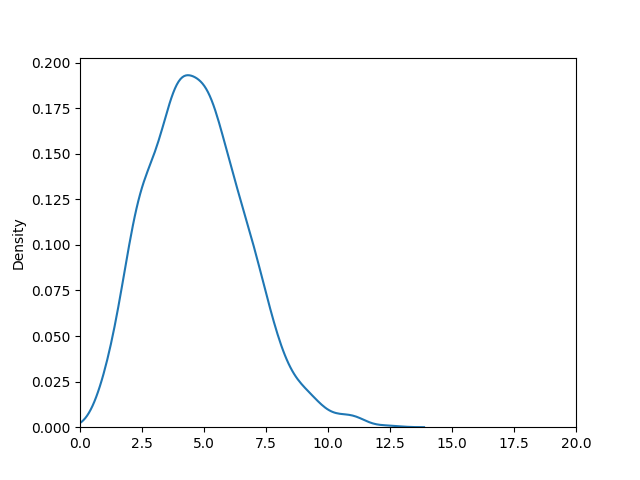
\includegraphics[scale=1.2]{HW1/Maxwell/3_Model/Maxwell.png}
    \end{center}
    \\
    \textbf{\textit{Листинг кода:}}
    \lstinputlisting[language=Python]{HW1/Maxwell/3_Model/maxwell.py}
	
	
	\chapter{Основные понятия математической статистики}
	
	\section{Биномиальное распределение}
	\subsection{Генерация выборок}
	В данном разделе производится генерация выборок объёмов 5, 10, 100, 200, 400, 600, 800, 1000 биномиального распределения с параметрами $\displaystyle n = 87, \theta = 0.6$ \\
	
	\textbf{5} \\
	\begin{center}
	   \fbox{53 59 60 49 51} \\
	   \caption{Таблица 1.1: выборка из Биномиального распределения, n = 5}
	\end{center}
	\\
	\\
	
	\textbf{10} \\
	\begin{center}
	   \fbox{58 50 52 54 48 53 51 55 51 48} \\
	   \caption{Таблица 1.2: выборка из Биномиального распределения, n = 10}
	\end{center}
	\newpage
	
	\textbf{100} \\
	\begin{figure}[h]
        \centering
        \fbox{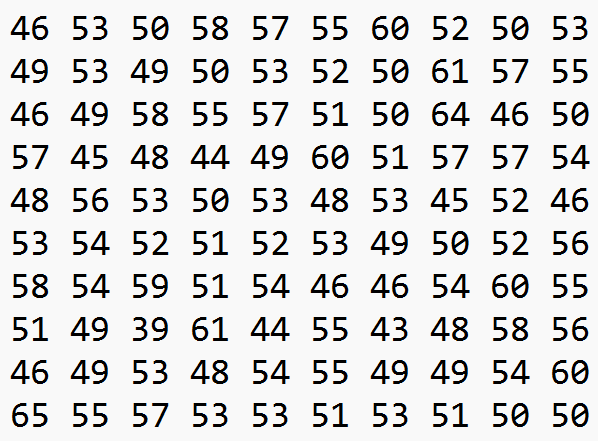
\includegraphics[scale=0.7]{HW2/Binomial/1_Selections/Binomial_100.png}}
        \caption{Таблица 1.3: выборка из Биномиального распределения, n = 100}
        \label{fig:my_label}
    \end{figure}

	\textbf{200} \\
	\begin{figure}[h]
        \centering
        \fbox{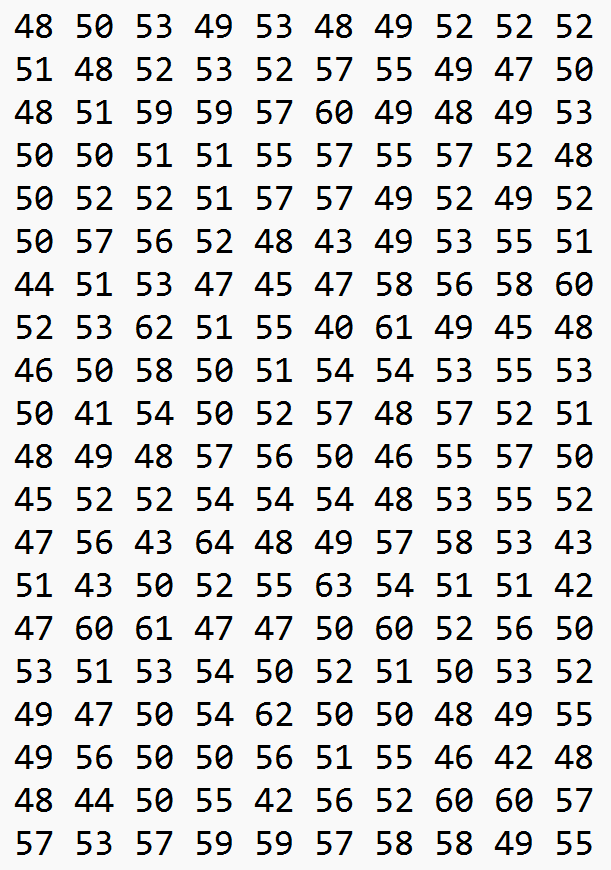
\includegraphics[scale=0.7]{HW2/Binomial/1_Selections/Binomial_200.png}}
        \caption{Таблица 1.4: выборка из Биномиального распределения, n = 200}
        \label{fig:my_label}
    \end{figure}

	\newpage
	\textbf{400} \\
	\begin{figure}[h]
        \centering
        \fbox{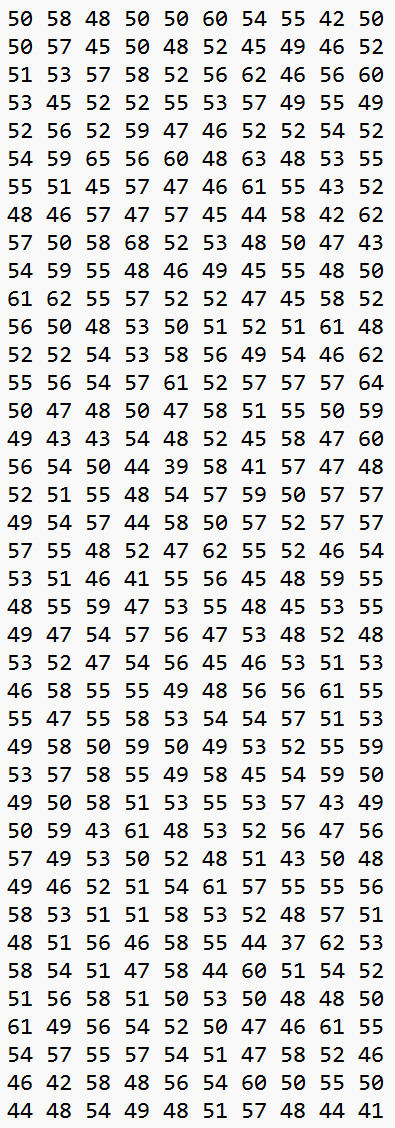
\includegraphics[scale=0.7]{HW2/Binomial/1_Selections/Binomial_400.png}}
        \caption{Таблица 1.5: выборка из Биномиального распределения, n = 400}
        \label{fig:my_label}
    \end{figure}

	\newpage
	\textbf{600} \\
	\begin{figure}[h]
        \centering
        \fbox{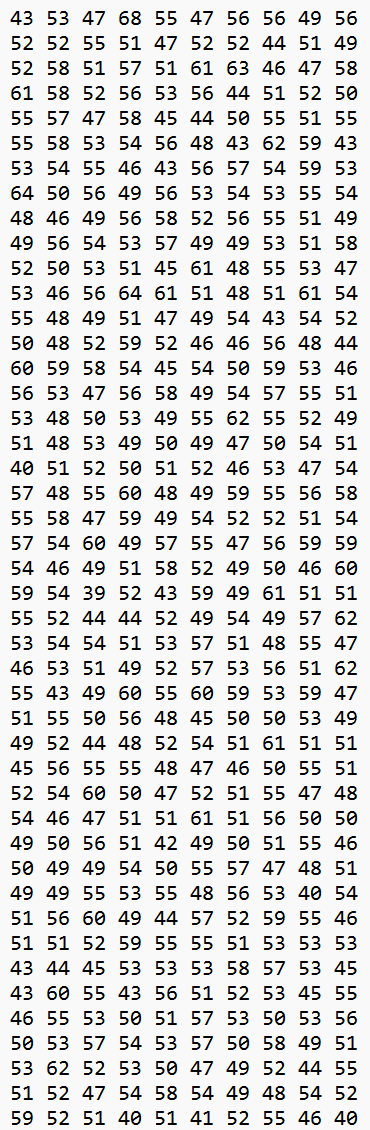
\includegraphics[scale=0.7]{HW2/Binomial/1_Selections/Binomial_601.png}}
        \fbox{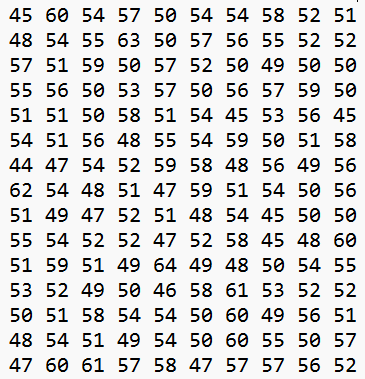
\includegraphics[scale=0.7]{HW2/Binomial/1_Selections/Binomial_602.png}}
        \caption{Таблица 1.6: выборка из Биномиального распределения, n = 600}
        \label{fig:my_label}
    \end{figure}

	\newpage
	\textbf{800} \\
	\begin{figure}[h]
        \centering
        \fbox{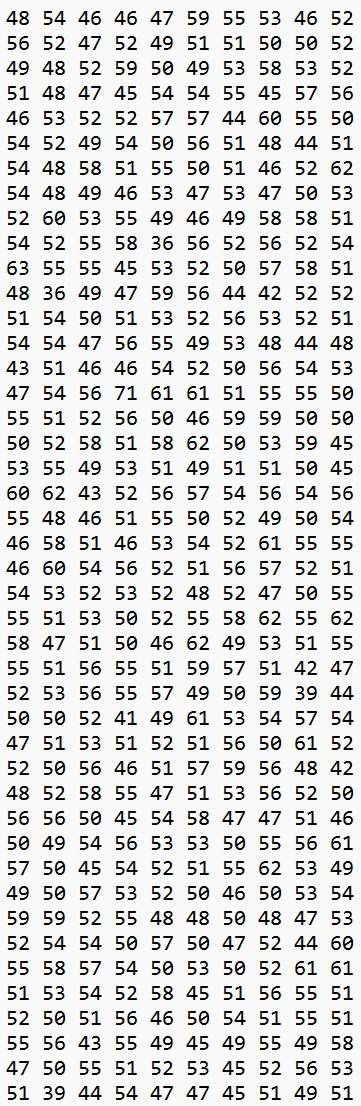
\includegraphics[scale=0.7]{HW2/Binomial/1_Selections/Binomial_801.png}}
        \fbox{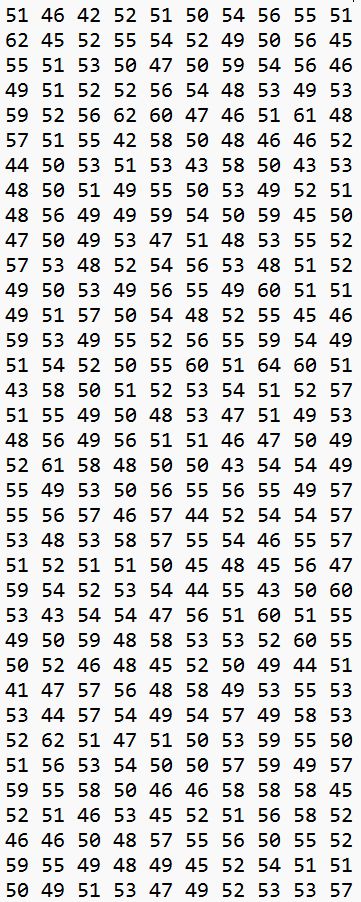
\includegraphics[scale=0.7]{HW2/Binomial/1_Selections/Binomial_802.png}}
        \caption{Таблица 1.7: выборка из Биномиального распределения, n = 800}
        \label{fig:my_label}
    \end{figure}

	\newpage
	\textbf{1000} \\
	\begin{figure}[h]
        \centering
        \fbox{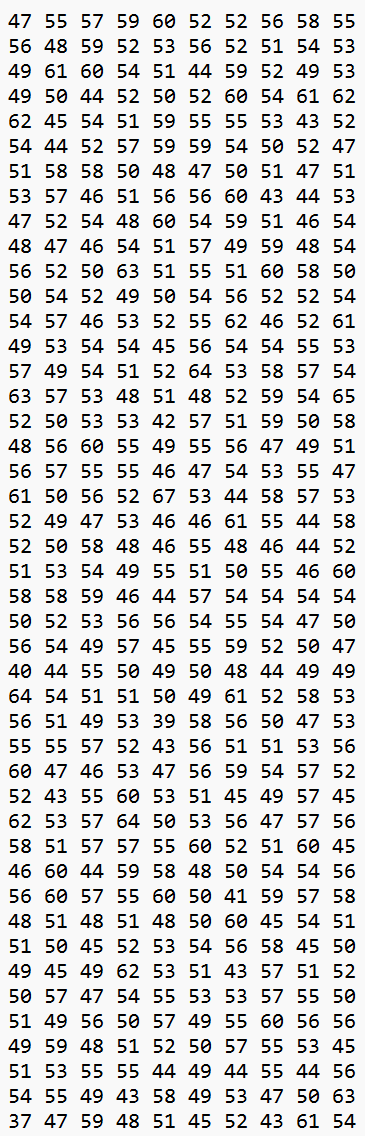
\includegraphics[scale=0.7]{HW2/Binomial/1_Selections/Binomial_1001.png}}
        \fbox{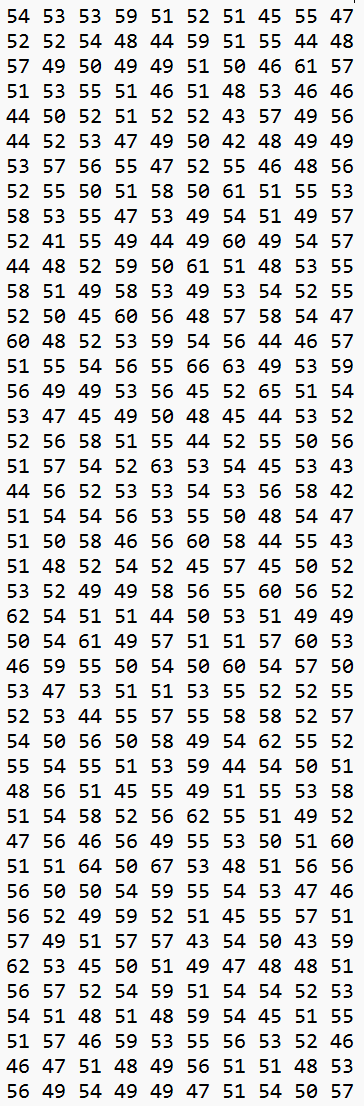
\includegraphics[scale=0.7]{HW2/Binomial/1_Selections/Binomial_1002.png}}
        \fbox{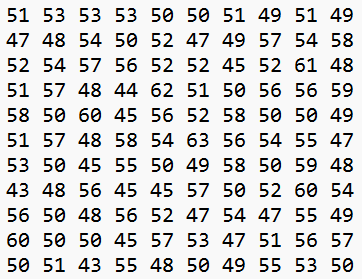
\includegraphics[scale=0.7]{HW2/Binomial/1_Selections/Binomial_1003.png}}
        \caption{Таблица 1.8: выборка из Биномиального распределения, n = 1000}
        \label{fig:my_label}
    \end{figure}
	\\
	\newpage
	\subsection{Построение эмпирической функции распределения}
	Из \textbf{\textit{Определения 1.11}}[\textit{\textbf{22} - Фомин Д. Б, Чухно А. Б., "Математическая статистика. Курс лекций для студентов кафедры компьютерной безопасности": \textbf{стр. 7}}]
	можем видеть, что:\\
	Пусть $X$ - некоторая выборка\\
	$\displaystyle\mu_{n}(y) = \sum_{i=1}^{n}Ind(X_{i} \leq y), y \in \mathbb{R}$ - случайная величина, равная числу элементов выборки $X$ меньших или равных $y$. Тогда функцию:
	\begin{center}
	    $\displaystyle \widehat{F}_{n}(y) = \frac{\mu_{n}(y)}{n}$
	\end{center}
	Будем называть Эмпирической Функцией Распределения, соответствующей выборке $X$. \\
	Эмпирическая кумулятивная функция распределения, возвращающая на основе выборки и числа t долю значений в выборке, меньших t, представлена в листинге ниже (под именем \textit{CDF}). \\
	\textbf{\textit{Листинг кода:}}
    \lstinputlisting[language=Python]{HW2/Binomial/2_EmpFuncs/EmpBin.py}

    Ниже представлены графики Эмпирической Функции Распределения для каждой выборки с графиками функции распределения случайной величины:\\
    Также, проанилизировав приведённые графики, можно сделать вывод, что при увеличении объёма выборки график кумулятивной эмпирической функции распределения всё больше "стремится" к графику функции распределения случайной величины. Также это подтверждается \textbf{\textit{Теоремой}} [\textit{\textbf{23} - Фомин Д. Б, Чухно А. Б., "Математическая статистика. Курс лекций для студентов кафедры компьютерной безопасности": \textbf{стр. 8}}], гласящей о том, что:\\
    \begin{center}
        $\displaystyle \textrm{Для } \forall x \in \mathbb{R} \textrm{ и для } \forall \epsilon>0 \textrm{ при } n \longrightarrow \infty \\
        \displaystyle P\Big(\Big|\widehat{F}_{n}(x) - F(x)\Big| < \epsilon\Big) \longrightarrow 1$
    \end{center}
    Другими словами: для произвольного фиксированного $y \in \mathbb{R}$ э.ф.р. $\widehat{F}_{n}(y)$ с увеличением объема выборки $n$ стремится к значению функции распределения $F(y)$.

    \begin{center}
        \fbox{\includegraphics[scale=1]{HW2/Binomial/2_EmpFuncs/5.png}}
        \fbox{\includegraphics[scale=1]{HW2/Binomial/2_EmpFuncs/10.png}}
        \fbox{\includegraphics[scale=1]{HW2/Binomial/2_EmpFuncs/100.png}}
        \fbox{\includegraphics[scale=1]{HW2/Binomial/2_EmpFuncs/200.png}}
        \fbox{\includegraphics[scale=1]{HW2/Binomial/2_EmpFuncs/400.png}}
        \fbox{\includegraphics[scale=1]{HW2/Binomial/2_EmpFuncs/600.png}}
        \fbox{\includegraphics[scale=1]{HW2/Binomial/2_EmpFuncs/800.png}}
        \fbox{\includegraphics[scale=1]{HW2/Binomial/2_EmpFuncs/1000.png}}
    \end{center}

    Для посчета $D_{n, m}$ необходимо описать функцию супремума, которая описана ниже:
    \lstinputlisting[language=Python]{HW2/Binomial/2_Dnm/BinSup.py}
    
    Описав функцию супремума, опишем и саму функцию подсчета $D_{n, m}$: 
    \lstinputlisting[language=Python]{HW2/Binomial/2_Dnm/Dnm.py}
    
    Произведём расчёты функции $D_{n,m}$ для каждой пары выборок с помощью скрипта на языке Python. Получим матрицу значений, которая, что примечательно, симметрична относительно главной диагонали.
    
    \begin{center}
        \fbox{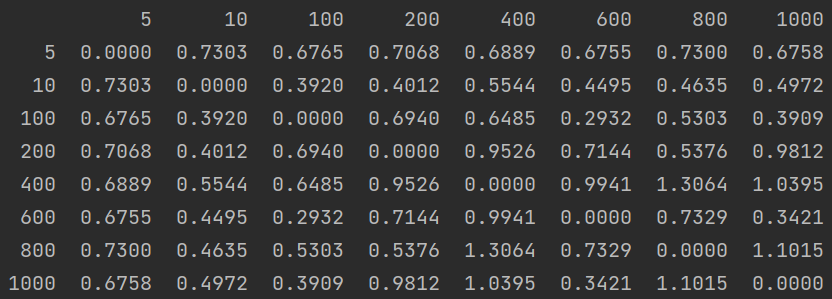
\includegraphics[scale=1]{HW2/Binomial/2_Dnm/BinDnm.png}}
    \end{center}

  \subsection{Построение гистограммы частот}
  Ниже представлены гистограммы частот для каждой выборки с графиками функции вероятности: \\
  Из приведенных ниже гистограмм частот можно сделать вывод, что с увеличением объёма выборки - её гистограмма частот "стремится" к функции вероятности. Это иллюстрирует следующую теорему:\\
      
      [\textit{\textbf{24} - Н. И. Чернова, "Лекции по математической статистике", Нижегородский Государственный Университет: \textbf{стр. 12, стр. 20}}] Пусть распределение $F$ абсолютно непрерывно, $f$ - его истинная плотность. Пусть, кроме того, число $k$ интервалов группировки не зависит от $n$. Тогда справедлива Теорема:\\
      \begin{center}
          При $\displaystyle n \longrightarrow \infty \textrm{  } \forall j = 1,\cdots,k \\
          \displaystyle l_{j}\cdot f_{j} = \frac{v{i}}{n} \longrightarrow^{p} P(X_{1} \in A_{j}) = \int_{A_{j}}f(\chi)d\chi$
      \end{center}
    Предполагаемую область значений случайной величины $\xi$ делят независимо от выборки на некоторое количество интервалов (не обязательно одинаковых). Пусть $A_{1},\cdots, A_{k}$ - интервалы на прямой, называемые интервалами группировки. Обозначим для $j = 1,\cdots,k$ через $v_{j}$ число элементов выборки, попавших в интервал $A_{j}$. $l_{j}$ - длина интервала $A_{j}$\\
    Данная теорема утверждает, что площадь столбца гистограммы, построенного над интервалом группировки, с ростом объема выборки сближается с площадью области под графиком плотности над этим же интервалом.
  \begin{center}
        \fbox{\includegraphics[scale=1]{HW2/Binomial/3_HISTS/1.png}}
        \fbox{\includegraphics[scale=1]{HW2/Binomial/3_HISTS/10.png}}
        \fbox{\includegraphics[scale=1]{HW2/Binomial/3_HISTS/100.png}}
        \fbox{\includegraphics[scale=1]{HW2/Binomial/3_HISTS/200.png}}
        \fbox{\includegraphics[scale=1]{HW2/Binomial/3_HISTS/400.png}}
        \fbox{\includegraphics[scale=1]{HW2/Binomial/3_HISTS/600.png}}
        \fbox{\includegraphics[scale=1]{HW2/Binomial/3_HISTS/800.png}}
        \fbox{\includegraphics[scale=1]{HW2/Binomial/3_HISTS/1000.png}}
    \end{center}

    \textbf{Листинг кода:} \\
    \lstinputlisting[language=Python]{HW2/Binomial/3_HISTS/BinHist.py}
    
    \newpage
    \subsection{Вычисление выборочных моментов}
    Оценка математического ожидания является \textbf{несмещенной} и \textbf{состоятельной}\\
    Оценка дисперсии является \textbf{смещенной} и \textbf{состоятельной}\\
    Докажем эти факты: \\
    \textbf{Доказательство несмещённости оценки математического ожидания} \\
    По \textit{\textbf{Определению 2.6}} [\textit{\textbf{25} - Фомин Д. Б, Чухно А. Б., "Математическая статистика. Курс лекций для студентов кафедры компьютерной безопасности": \textbf{стр. 12}}] знаем, что, если смещение $b(\theta)$ равно нулю, то оценка является \textbf{несмещённой}, где
    \begin{center}
        $\displaystyle b(\theta) = M_{\theta}T(X) - \tau(\theta)$
    \end{center}
    Таким образом, в случае выборочного среднего, имеем:
    \begin{center}
        $\displaystyle \tau(\theta) = MX_{i}, i = 1,\cdots,n \\
        \displaystyle \overline{X} = T(X) = \frac{1}{n}\sum_{i=1}^{n}X_{i}, n$ - объём выборки. 
    \end{center}
    Найдем математическое ожидание выборочного среднего: \\
    $\displaystyle MT(X) = \frac{1}{n}M\sum_{i=1}^{n}X_{i} = \frac{1}{n}\sum_{i=1}^{n}M X_{i} = \frac{1}{n}nMX_{i} = MX_{i}$ \\
    Из приведенного доказательства видно, что \\
    $\displaystyle b(\theta) = M_{\theta}T(X) - \tau(\theta) = MX_{i} - MX_{i} = 0$\\
    Следовательно, оценка является \textbf{несмещённой}.\\
    
    \textbf{Доказательство состоятельности оценки математического ожидания}\\
    Воспользуемся утверждением [\textit{\textbf{26} - Фомин Д. Б, Чухно А. Б., "Математическая статистика. Курс лекций для студентов кафедры компьютерной безопасности": \textbf{стр. 15}}] о том, что для проверки состоятельности несмещенной оценки достаточно убедиться в том, что ее дисперсия стремится к 0 при n, стремящемуся к $\infty$.\\
    Также воспользуемся \textit{\textbf{Свойством 4}} [\textit{\textbf{27} - Фомин Д. Б, Чухно А. Б., "Теория Вероятности. Курс лекций для студентов кафедры компьютерной безопасности": \textbf{стр. 72}}], которое гласит, что:
    \begin{center}
        $\displaystyle D(c \cdot \xi) = x^{2} \cdot D\xi$
    \end{center}
    Таким образом: \\
    $\displaystyle DT(X) = D\Big(\frac{1}{n} \cdot \sum_{i=1}^{n}M X_{i}\Big) = \frac{1}{n^2}\Big(\sum_{i=1}^{n}D X_{i}\Big) = \frac{1}{n^2}nDX_{i} = \frac{1}{n}DX_{i}$\\
    Тогда: \\
    $\displaystyle \lim_{n \longrightarrow \infty}DT(X) = \frac{1}{n}DX_{i} = 0$ \\
    т.к. $\displaystyle\frac{1}{n^2} \longrightarrow 0 \textrm{ при } n \longrightarrow \infty$\\
    Тогда, можем сделать вывод, что оценка выборочного среднего \textbf{несмещённая} и \textbf{состоятельная}.\\
    
    \textbf{Доказательство смещенности оценки дисперсии}\\
    Воспользуемся тем же утверждением, что и в доказательстве несмещенности оценки выборочного среднего. А также воспользуемся утверждениями с уже упомянтой \textbf{\textit{стр. 12}} лекций курса Математической статистики. Тогда:\\
    \begin{center}
        $\displaystyle \textrm{Пусть } Y_{i} = X_{i} - a_{1}, a_{1} = M\xi (1)\\
        \displaystyle \textrm{Следовательно: } \overline{Y} = \overline{X} - M\overline{X} (2) \\
        $
    \end{center}
    Тогда: \\
    $\displaystyle MT(X) = \frac{1}{n}M\sum_{i=1}^{n}(Y_{i}-\overline{Y})^{2} =$ по определению: $\overline{Y} = \sum_{j = 1}^{n}Y_{j}$, поэтому $\displaystyle =\\= \frac{1}{n}M\sum_{i=1}^{n}(Y_{i}^{2} + \overline{Y}^{2} - 2\Big(\frac{1}{n}\sum_{j = 1}^{n}Y_{j}\Big)Y_{i}) = \frac{1}{n}M\Big(\sum_{i=1}^{n}Y_{i}^{2} + \sum_{i=1}^{n}\overline{Y}^{2} - 2\Big(\frac{1}{n}\sum_{i, j = 1}^{n}Y_{j}Y_{i}\Big)\Big) =\\= \frac{1}{n}\Big(\sum_{i=1}^{n}MY_{i}^{2} + \sum_{i=1}^{n}M\overline{Y}^{2} - \frac{2}{n}\sum_{i, j = 1}^{n}M(Y_{j}Y_{i})\Big) = $ 
    \\
    \begin{tcolorbox}
        \textbf{Установим следующие факты:}\\
        \textbf{\textit{1}}. $\displaystyle MY_{i} =$ опираясь на утверждение (1) $= MX_{i} - M(MX_{i}) = $ Мат ожидание - константа. Мат ожидание константы равна этой же константе, следовательно $= MX_{i} - MX_{i} = 0$\\
        \textbf{\textit{2}}. $\displaystyle MY_{i}^{2} =$ вычтем из Мат. Ожидания нулевую величину $=\\= MY_{i}^{2} - (MY_{i})^{2} = DY_{i}$\\
        \textbf{\textit{3}}. Если $i \neq j$, то верно следующее:\\
        $\displaystyle M(Y_{i}Y_{j}) = MY_{i}MY_{j}$\\
        Учитывая пункт \textbf{1} ($MY_{i} = 0$), получим:\\
        $\displaystyle M(Y_{i}Y_{j}) = MY_{i}MY_{j} = 0$\\
        \end{tcolorbox}
        \begin{tcolorbox}
        \textbf{\textit{4}}. $\displaystyle M\overline{Y}^{2} = \frac{1}{n^2}\sum_{i, j = 1}^{n}M(Y_{i}Y_{j}) = $ имеем сумму сумм $= \displaystyle\frac{1}{n^2}\Big(\sum_{i \neq j}M(Y_{i}Y_{j}) +\\+ \sum_{i = 1}^{n}MY_{i}^{2}\Big) = $ опираясь на пункт \textbf{3}, значем, что $M(Y_{i}Y_{j}) = 0$, тогда $= \frac{1}{n^2}\sum_{i = 1}^{n}MY_{i}^{2} = $ опираясь на пункт \textbf{2}, знаем, что $MY_{i}^{2} = DY_{i}$, тогда $= \displaystyle\frac{1}{n^2}\sum_{i=1}^{n}DY_{i} = \frac{1}{n^2}nDY_{i}= \frac{1}{n}DY_{i}$
        \end{tcolorbox}
    $\displaystyle = \frac{1}{n}\Big(\Big(1 - \frac{2}{n}\Big)\sum_{i = 1}^{n}MY_{i}^{2} + \sum_{i = 1}^{n}M\overline{Y}^{2}\Big) = \frac{1}{n}\Big((1 - \frac{2}{n}\Big)nDY_{i} + DY_{i}\Big) =\\= \frac{1}{n}\Big(DY_{i}\Big(n + 1 - 2\Big)\Big) = \frac{n - 1}{n}DY_{i} = \frac{n - 1}{n}D(X_{i} - MX_{i}) = $ Опираясь на то, что $\displaystyle D(\xi + c) = D\xi$, получаем $\displaystyle = \frac{n - 1}{n}DX_{i}$
    \\
    Таким образом, $\displaystyle b(\theta) = DX_{i} - \frac{n - 1}{n}DX_{i} \neq 0$\\
    Следовательно, оценка дисперсии \textbf{смещённая}.\\
    
    \textbf{Доказательство состоятельности оценки дисперсии}\\
    По определению: $\displaystyle \overline{S}^{2} = \frac{1}{n}\sum_{i = 1}^{n}(X_{i} + \overline{X})^{2} = \frac{1}{n}\sum_{i = 1}^{n}(X_{i}^{2} + (\overline{X})^{2} - 2X_{i}\overline{X}) = \frac{1}{n}\sum_{i=1}^{n}X_{i}^{2} -\\- \frac{2}{n}\overline{X}\sum_{i=1}^{n}X_{i} + \frac{1}{n}(\overline{X})^{2}\sum_{i=1}^{n} = \overline{X^{2}} - 2\overline{X}\cdot\overline{X} + (\overline{X})^{2} = \overline{X^{2}} - (\overline{X})^{2}$\\
    Тогда, опираясь на вышеописанные записи и Закон Больших Чисел в форме Хинчина [\textit{\textbf{28} - \href{http://angtu.ru/universitet/kafedry-angtu/math/posobiya/metTV_ch_2.pdf}{Источник, \textbf{стр. 77}}}], получим, что:\\
    $\displaystyle\overline{X}^{2} - (\overline{X})^{2} \longrightarrow_{n \longrightarrow \infty}^{p} MX_{i}^{2} - (MX_{i})^{2} = DX_{i}$\\
    Таким образом, оценка дисперсии \textbf{состоятельна}.\\
    
    Истинное выборочное среднее при параметрах $\displaystyle n = 87, \theta = 0.6$:\\
    $\displaystyle n \cdot \theta = 87 \cdot 0.6 = 52.2$\\
    Истинное выборочная дисперсия при параметрах $\displaystyle n = 87, \theta = 0.6:$\\
    $\displaystyle n \cdot \theta \cdot (1 - \theta) = 87 \cdot 0.6 \cdot 0.4 = 20.88$
    \\
    \begin{center}
        \includegraphics[scale = 1.2]{HW2/Binomial/4_1/1.png}
    \end{center}
    Вычислим погрешность выборочного среднего и выборочной дисперсии, зная истинные значения данных величин:
    \begin{center}
        \includegraphics[scale = 1.2]{HW2/Binomial/4_1/2.png}
    \end{center}
    \textbf{Листинг кода:}
    \lstinputlisting[language=Python]{HW2/Binomial/4_1/BinMoments.py}
    
    \section{Распределение Максвелла}
    \subsection{Генерация выборок}
    В данном разделе производится генерация выборок объёмов 5, 10, 100, 200, 400, 600, 800, 1000 распределения Максвелла с параметром $\theta = 3$\\
    \textbf{5}\\
    \begin{center}
        \fbox{5.978659 3.882685 5.332642 3.792912 2.248517}\\
        Выборка из распределения Максвелла, n = 5
    \end{center}
    
    \textbf{10}\\
    \begin{center}
        \fbox{2.437915 2.313844 4.983702 5.628353 3.314616 4.39135 2.641108 4.972171 4.316611 5.1504}\\
        Выборка из распределения Максвелла, n = 10
    \end{center}
    
    \newpage
    \textbf{100}\\
    \begin{center}
        \fbox{\includegraphics[scale = 1]{HW2/Maxwell/1_Selections/100.png}}
        Выборка из распределения Максвелла, n = 100
    \end{center}
    
    \textbf{200}\\
    \begin{center}
        \fbox{\includegraphics[scale = 1]{HW2/Maxwell/1_Selections/200.png}}
        Выборка из распределения Максвелла, n = 200
    \end{center}
    
    \newpage
    \textbf{400}\\
    \begin{center}
        \fbox{\includegraphics[scale = 1]{HW2/Maxwell/1_Selections/400.png}}
        Выборка из распределения Максвелла, n = 400
    \end{center}
    
    \newpage
    \textbf{600}\\
    \begin{center}
        \fbox{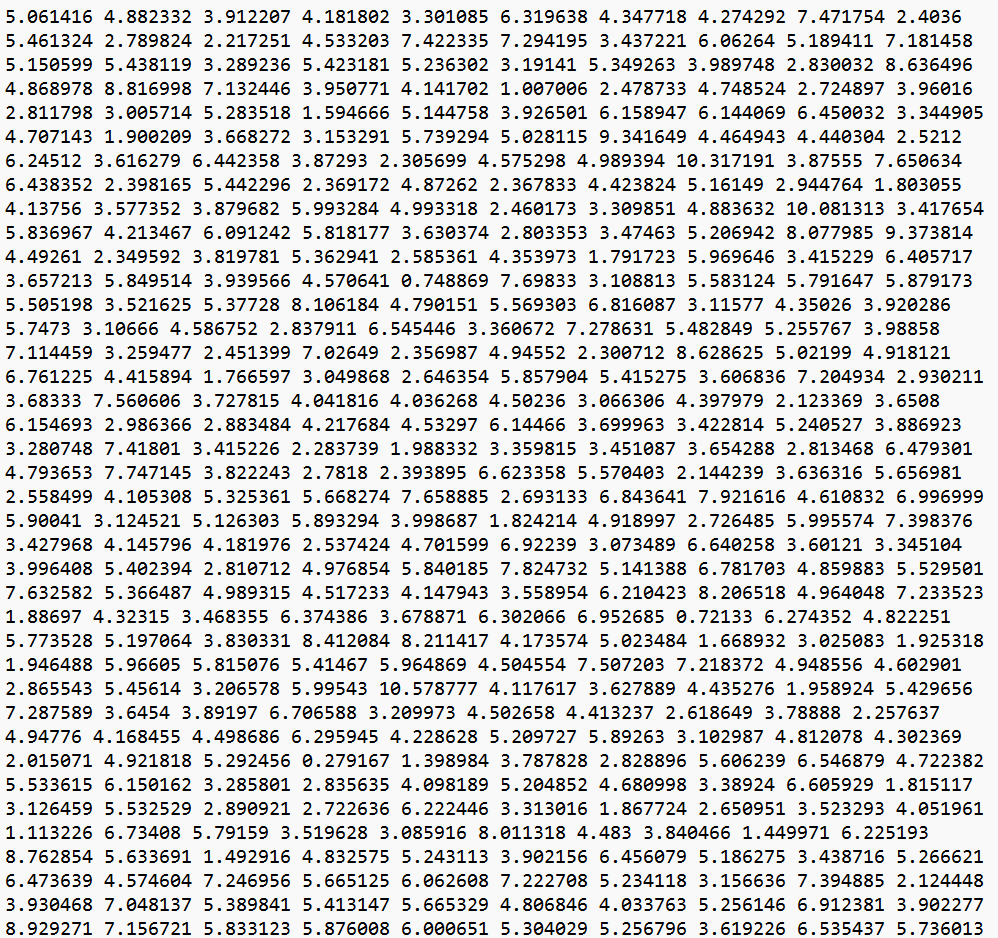
\includegraphics[scale = 1]{HW2/Maxwell/1_Selections/601.png}}
        \fbox{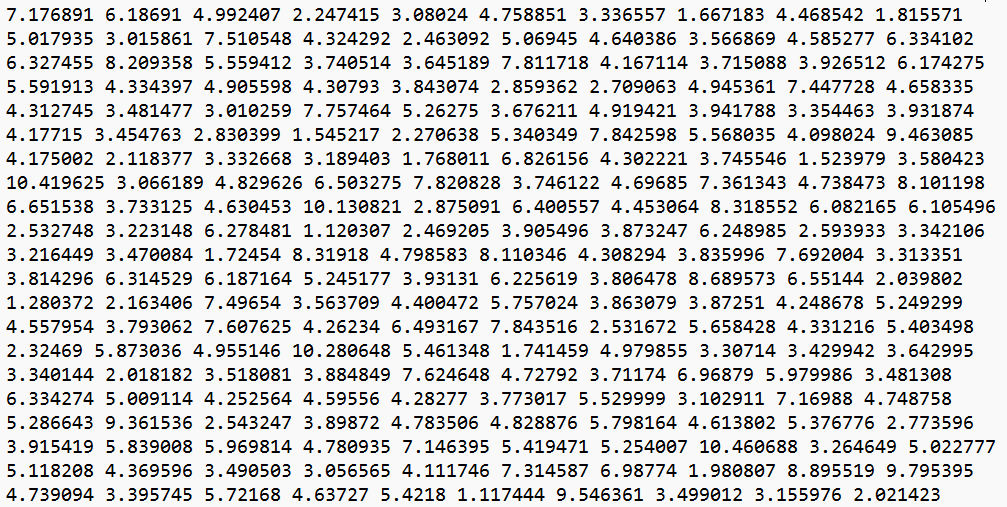
\includegraphics[scale = 1]{HW2/Maxwell/1_Selections/602.png}}
        Выборка из распределения Максвелла, n = 600
    \end{center}
    
    \newpage
    \textbf{800}\\
    \begin{center}
        \fbox{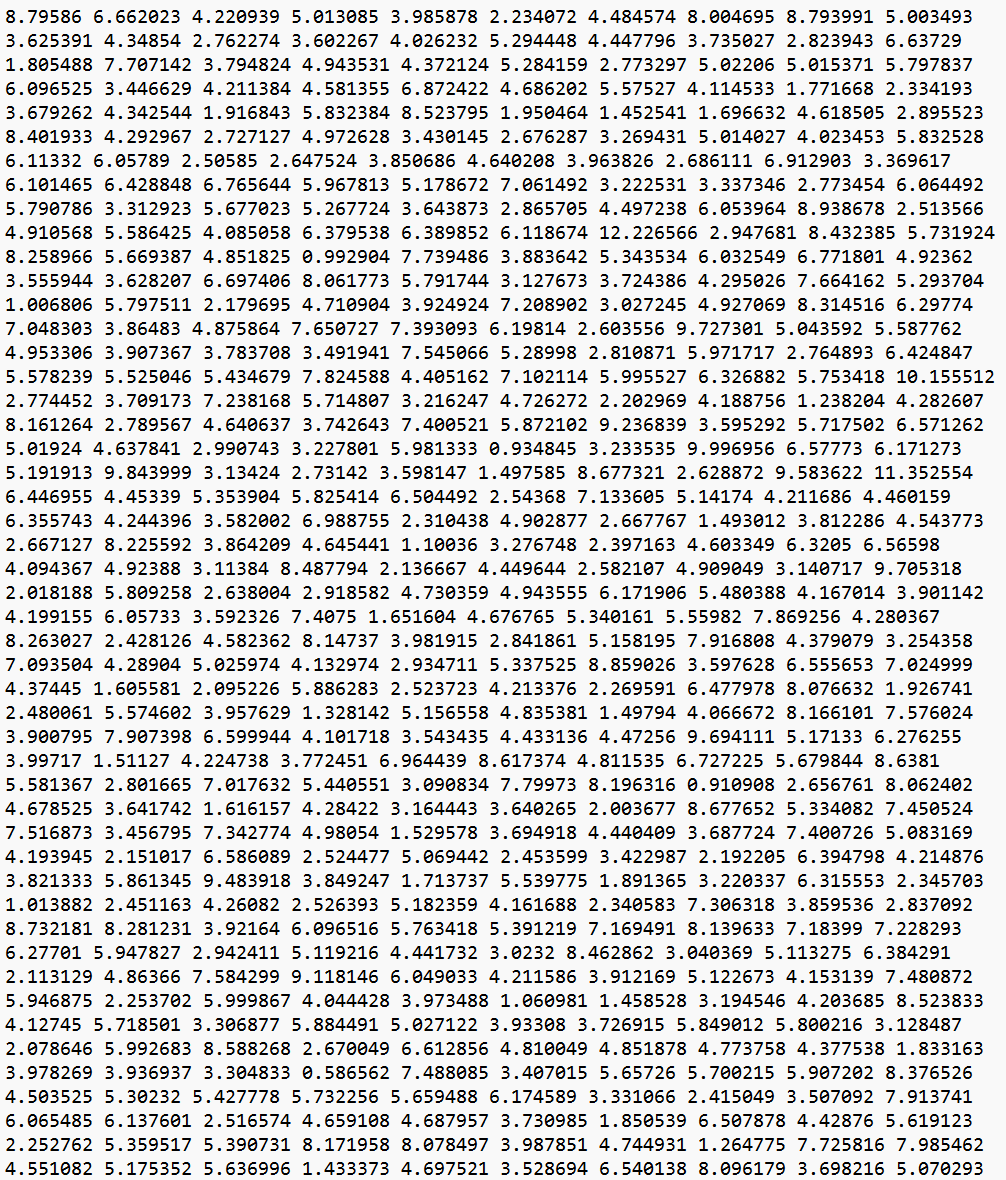
\includegraphics[scale = 1]{HW2/Maxwell/1_Selections/801.png}}
        \fbox{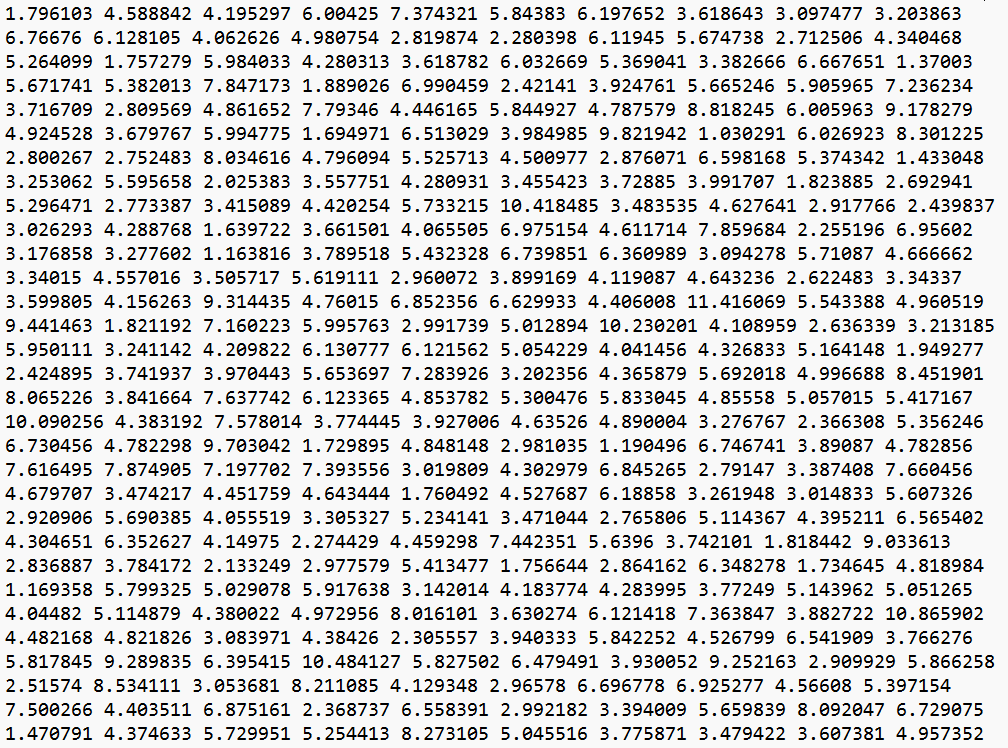
\includegraphics[scale = 1]{HW2/Maxwell/1_Selections/802.png}}
        Выборка из распределения Максвелла, n = 800
    \end{center}
    
    \newpage
    \textbf{1000}\\
    \begin{center}
        \fbox{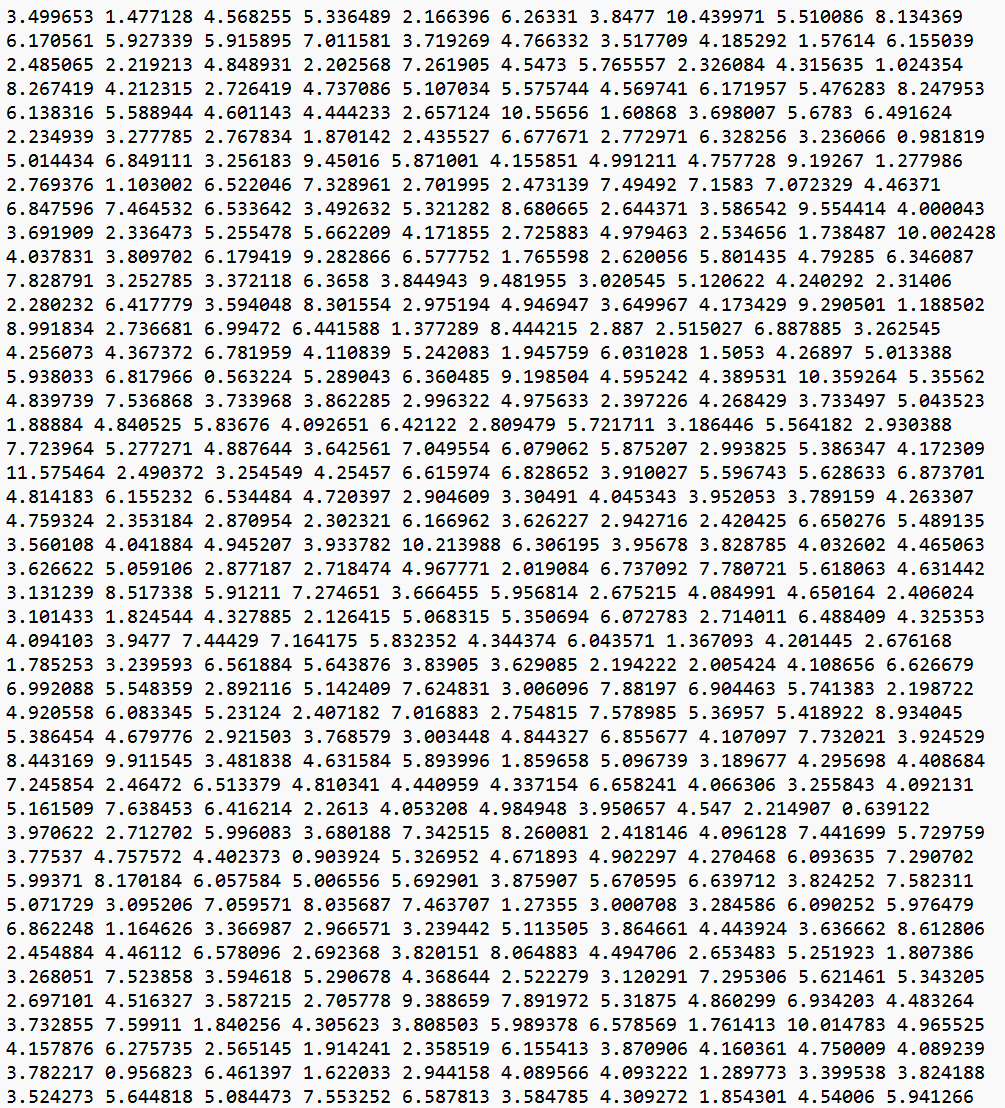
\includegraphics[scale = 1]{HW2/Maxwell/1_Selections/1001.png}}
        \fbox{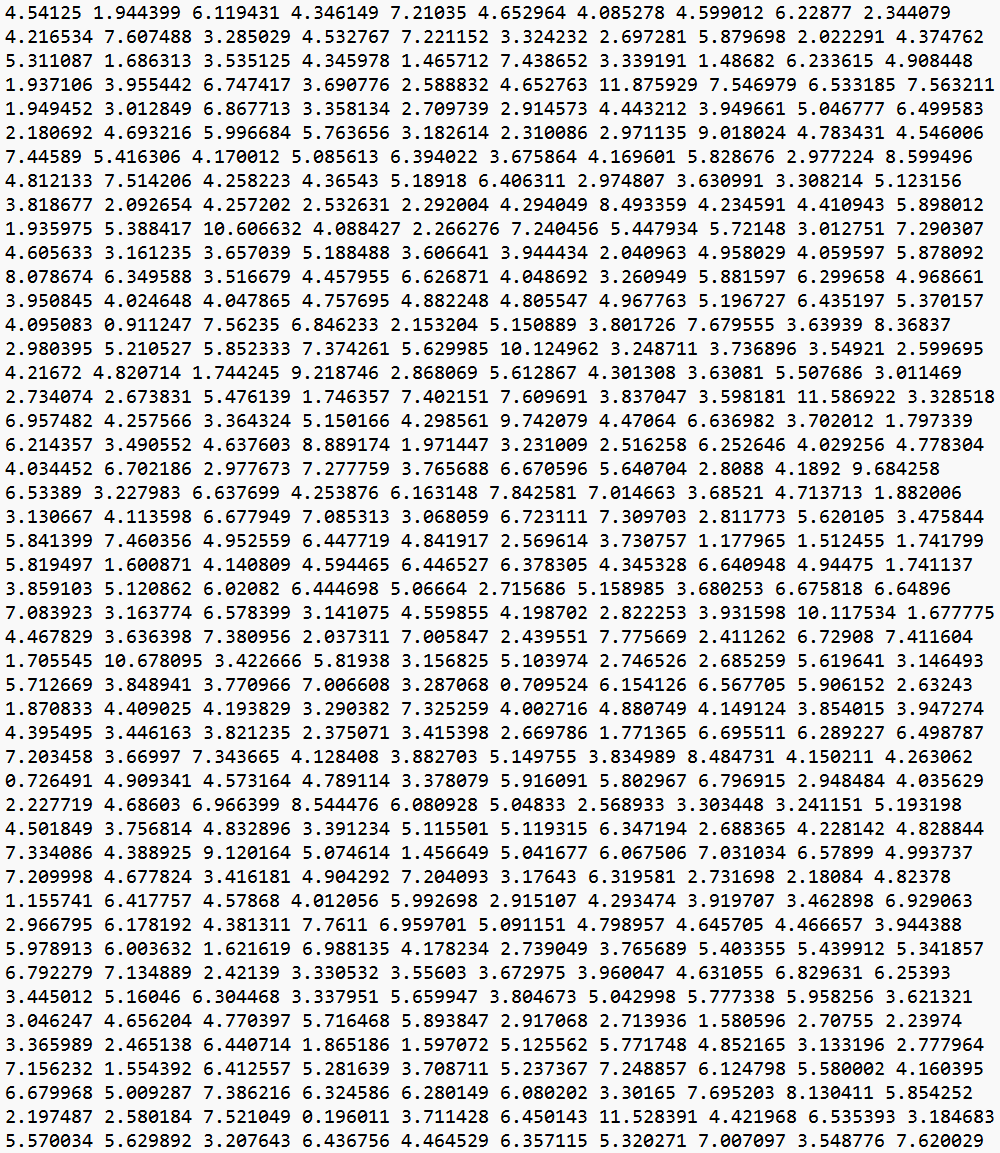
\includegraphics[scale = 1]{HW2/Maxwell/1_Selections/1002.png}}
        \fbox{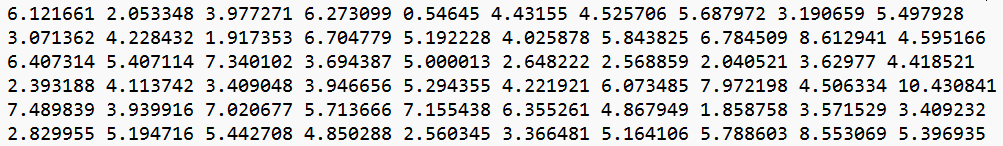
\includegraphics[scale = 1]{HW2/Maxwell/1_Selections/1003.png}}
        Выборка из распределения Максвелла, n = 1000
        
    \end{center}
    
    \subsection{Построение эмпирической функции распределения}
    Опираясь на утверждения об Эмпирической Функции Распределения из пункта \textbf{2.1.2}, построим графики ЭФР.
    Эмпирическая кумулятивная функция распределения, возвращающая на основе выборки и числа t долю значений в выборке, меньших t, представлена в листинге ниже (под именем \textit{CDF}). \\
	\textbf{\textit{Листинг кода:}}
    \lstinputlisting[language=Python]{HW2/Maxwell/2_EmpFuncs/EmpMax.py}
    Ниже представлены графики Эмпирической Функции Распределения для каждой выборки с графиками функции распределения случайной величины:\\
    Также, проанилизировав приведённые графики, можно сделать вывод, что при увеличении объёма выборки график кумулятивной эмпирической функции распределения всё больше "стремится" к графику функции распределения случайной величины. Также это подтверждается \textbf{\textit{Теоремой}} [\textit{\textbf{29} - Фомин Д. Б, Чухно А. Б., "Математическая статистика. Курс лекций для студентов кафедры компьютерной безопасности": \textbf{стр. 8}}], гласящей о том, что:\\
    \begin{center}
        $\displaystyle \textrm{Для } \forall x \in \mathbb{R} \textrm{ и для } \forall \epsilon>0 \textrm{ при } n \longrightarrow \infty \\
        \displaystyle P\Big(\Big|\widehat{F}_{n}(x) - F(x)\Big| < \epsilon\Big) \longrightarrow 1$
    \end{center}
    Другими словами: для произвольного фиксированного $y \in \mathbb{R}$ э.ф.р. $\widehat{F}_{n}(y)$ с увеличением объема выборки $n$ стремится к значению функции распределения $F(y)$.
    \begin{center}
        \fbox{\includegraphics[scale=1]{HW2/Maxwell/2_EmpFuncs/5.png}}
        \fbox{\includegraphics[scale=1]{HW2/Maxwell/2_EmpFuncs/10.png}}
        \fbox{\includegraphics[scale=1]{HW2/Maxwell/2_EmpFuncs/100.png}}
        \fbox{\includegraphics[scale=1]{HW2/Maxwell/2_EmpFuncs/200.png}}
        \fbox{\includegraphics[scale=1]{HW2/Maxwell/2_EmpFuncs/400.png}}
        \fbox{\includegraphics[scale=1]{HW2/Maxwell/2_EmpFuncs/600.png}}
        \fbox{\includegraphics[scale=1]{HW2/Maxwell/2_EmpFuncs/800.png}}
        \fbox{\includegraphics[scale=1]{HW2/Maxwell/2_EmpFuncs/1000.png}}
    \end{center}
    
    Для посчета $D_{n, m}$ необходимо описать функцию супремума, которая описана ниже:
    \lstinputlisting[language=Python]{HW2/Binomial/2_Dnm/BinSup.py}
    
    Описав функцию супремума, опишем и саму функцию подсчета $D_{n, m}$: 
    \lstinputlisting[language=Python]{HW2/Binomial/2_Dnm/Dnm.py}
    
    Произведём расчёты функции $D_{n,m}$ для каждой пары выборок с помощью скрипта на языке Python. Получим матрицу значений, которая, что примечательно, симметрична относительно главной диагонали.
    
    \begin{center}
        \fbox{\includegraphics[scale=1]{HW2/Maxwell/2_Dnm/Dnm.png}}
    \end{center}
    
    \subsection{Построение гистограммы частот}
     Ниже представлены гистограммы частот для каждой выборки с графиками функции плотности распределения: \\
      Из приведенных ниже гистограмм частот можно сделать вывод, что с увеличением объёма выборки - её гистограмма частот "стремится" к функции плотности распределения. Это иллюстрирует следующую теорему:\\
      
      [\textit{\textbf{30} - Н. И. Чернова, "Лекции по математической статистике", Нижегородский Государственный Университет - \textbf{стр. 12, стр. 20}}] Пусть распределение $F$ абсолютно непрерывно, $f$ - его истинная плотность. Пусть, кроме того, число $k$ интервалов группировки не зависит от $n$. Тогда справедлива Теорема:\\
      \begin{center}
          При $\displaystyle n \longrightarrow \infty \textrm{  } \forall j = 1,\cdots,k \\
          \displaystyle l_{j}\cdot f_{j} = \frac{v{i}}{n} \longrightarrow^{p} P(X_{1} \in A_{j}) = \int_{A_{j}}f(\chi)d\chi$
      \end{center}
    Предполагаемую область значений случайной величины $\xi$ делят независимо от выборки на некоторое количество интервалов (не обязательно одинаковых). Пусть $A_{1},\cdots, A_{k}$ - интервалы на прямой, называемые интервалами группировки. Обозначим для $j = 1,\cdots,k$ через $v_{j}$ число элементов выборки, попавших в интервал $A_{j}$. $l_{j}$ - длина интервала $A_{j}$\\
    Данная теорема утверждает, что площадь столбца гистограммы, построенного над интервалом группировки, с ростом объема выборки сближается с площадью области под графиком плотности над этим же интервалом.
  \begin{center}
        \fbox{\includegraphics[scale=1]{HW2/Maxwell/3_HISTS/5.png}}
        \fbox{\includegraphics[scale=1]{HW2/Maxwell/3_HISTS/10.png}}
        \fbox{\includegraphics[scale=1]{HW2/Maxwell/3_HISTS/100.png}}
        \fbox{\includegraphics[scale=1]{HW2/Maxwell/3_HISTS/200.png}}
        \fbox{\includegraphics[scale=1]{HW2/Maxwell/3_HISTS/400.png}}
        \fbox{\includegraphics[scale=1]{HW2/Maxwell/3_HISTS/600.png}}
        \fbox{\includegraphics[scale=1]{HW2/Maxwell/3_HISTS/800.png}}
        \fbox{\includegraphics[scale=1]{HW2/Maxwell/3_HISTS/1000.png}}
    \end{center}

    \textbf{Листинг кода:} \\
    \lstinputlisting[language=Python]{HW2/Maxwell/3_HISTS/MaxHist.py}
    
    \newpage
    \subsection{Вычисление выборочных моментов}
    Оценка математического ожидания является несмещенной и состоятельной (факты, доказанные в пункте \textbf{2.1.4})\\
    Оценка дисперсии является смещенной и состоятельной (факты, доказанные в пункте \textbf{2.1.4})\\
    
    Истинное выборочное среднее при параметрах $\displaystyle \theta = 3$:\\
    $\displaystyle 2 \cdot \theta \cdot \sqrt{\frac{2}{\pi}} = 2 \cdot 3 \cdot \sqrt{\frac{2}{\pi}} = 4.787$\\
    Истинное выборочная дисперсия при параметрах $\displaystyle \theta = 3:$\\
    $\displaystyle \theta^{2} \cdot \Big(3 - \frac{8}{\pi} \Big) = 9 \cdot \Big(3 - \frac{8}{\pi} \Big) = 4.081$
    \\
    \begin{center}
        \includegraphics[scale = 1.2]{HW2/Maxwell/4_1/1.png}
    \end{center}
    Вычислим погрешность выборочного среднего и выборочной дисперсии, зная истинные значения данных величин:
    \begin{center}
        \includegraphics[scale = 1.2]{HW2/Maxwell/4_1/2.png}
    \end{center}
    \textbf{Листинг кода:}
    \lstinputlisting[language=Python]{HW2/Maxwell/4_1/MaxMoments.py}
\end{document}